% !TeX program = xelatex
% !TeX encoding = utf8
% !TeX root = SigSys1_HS22.tex

%% TODO: publish to CTAN
\documentclass[margin=normal]{tex/hsrzf}

%%%%%%%%%%%%%%%%%%%%%%%%%%%%%%%%%%%%%%%%%%%%%%%%%%%
% Packages

%% TODO: publish to CTAN
\usepackage{tex/hsrstud}

%% Language configuration
\usepackage{polyglossia}
\setdefaultlanguage[variant=swiss]{german}

%% License configuration
\usepackage[
    type={CC},
    modifier={by-nc-sa},
    version={4.0},
    lang={german},
]{doclicense}

%other Packages
\usepackage{multicol,multirow}
\usepackage[export]{adjustbox}
%amssymb,amsmath,fancybox,graphicx,color,lastpage,
%wrapfig,fancyhdr,hyperref,verbatim,floatflt,
%multicol,multirow,rotating,pdflscape,array,longtable

%%%%%%%%%%%%%%%%%%%%%%%%%%%%%%%%%%%%%%%%%%%%%%%%%%%
% Metadata

\course{Elektrotechnik}
\module{SigSys}
\semester{Herbstsemester 2022}

\authoremail{joel.leirer@ost.ch}
\author{\textsl{Joël Leirer} -- \texttt{\theauthoremail}}

% did someone help you with this work?
\contributors{

}

\title{\texttt{\themodule} Zusammenfassung}
\date{\thesemester}

%%%%%%%%%%%%%%%%%%%%%%%%%%%%%%%%%%%%%%%%%%%%%%%%%%%
% Document

\begin{document}

% use roman numberals for introductiory pages
\pagenumbering{roman}

\maketitle

% \begin{abstract}
% \end{abstract}

% show the names of the people who contributed to this document.
% \section*{Contributors}
% \thecontributors

\section*{Lizenz}
\doclicenseThis
\clearpage
\tableofcontents

% actual content
\clearpage
\setcounter{page}{1}
\pagenumbering{arabic}

\section{Signalklassen}
\begin{multicols}{2}
    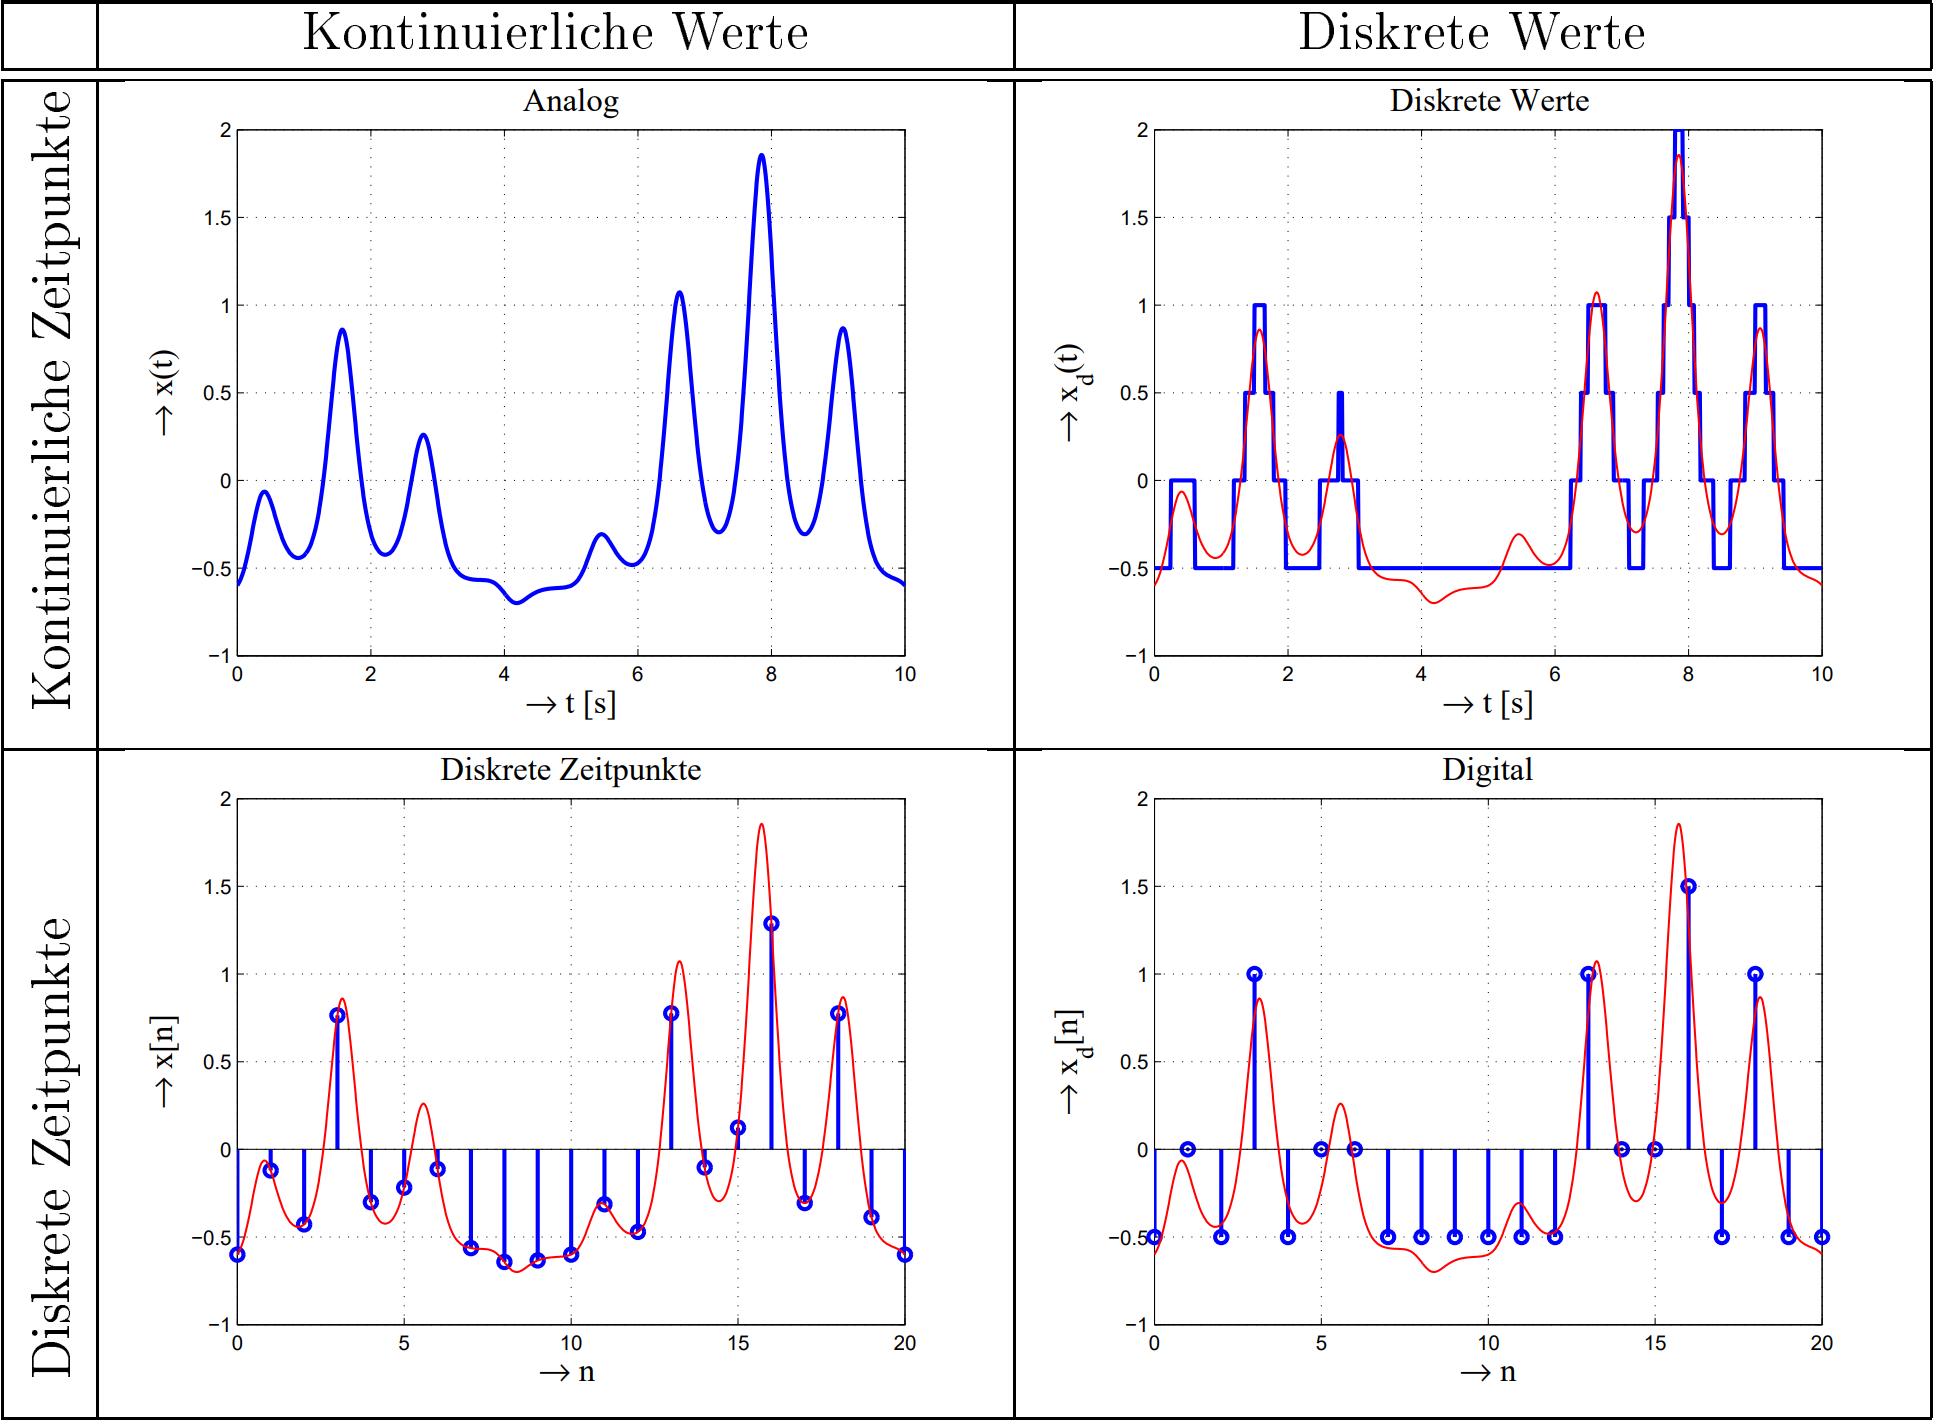
\includegraphics[width = 7cm]{include/Signalklassen/img/Signalklassen.png}
    \subsection{weitere Unterteilungen}
    \begin{tabular}{|c|c|}
        \hline
        Reellwertig $\mathbb{R}$ & Complexwertig $\mathbb{C}$ \\
        Eindimensional           & Mehrdimensional            \\
        Stochastisch             & Deterministisch            \\
        Energiesignale           & Leistungssignal            \\
        Analog                   & Digital                    \\
        Aperiodisch              & Periodisch                 \\
        \hline
    \end{tabular}
    \\[10pt]
    \begin{tabular}{|p{70pt}|p{70pt}|p{70pt}|}
        \hline
        Klasse 1            &
        Klasse 2a           &
        Klasse 2b                                                                          \\
        Energiesiegnal      & periodisches Leistungssignal & aperiodisches Leistungssignal \\
        $0 < W_n < \infty $ & $0 < P_n < \infty $          & $0 < P_n < \infty$            \\
        \hline
    \end{tabular}
\end{multicols}

\section{Kenngrössen von Signalen}
\begin{tabular}{p{6cm}p{12cm}}
  Energie                                                            &
  $W_n = \lim_{T \to \infty}  \int \limits _{-T/2} ^{T/2} |f(t)|^2 dt$            \\
  Leistung                                                           &
  $P_n = lim_{T \to \infty} \frac{1}{T} \int \limits _{-T/2} ^{T/2} |f(t)|^2 dt$  \\
  *Linearer Mittelwert
  \newline \tiny(auch: $ \bar{x}, x_m$)                              &
  $X_0 = \frac{1}{T} \int \limits _{-T/2}^{T/2} x(t) dt $                         \\
  *Quadratischer Mittelwert                                          &
  $X^2 = \frac{1}{T} \int \limits _{-T/2}^{T/2} x^2(t) dt$                        \\
  *Effektivwert \newline \tiny{("Quadratischer Mittelwert", RMS)}    &
  $X^2 = \frac{1}{T} \int \limits _{-T/2}^{T/2} \sqrt{x^2(t)} dt $                \\
  Mittelwert n. Ordnung \newline \tiny(nur Signale $\in \mathbb{R}$) &
  $X^n = \frac{1}{T} \int \limits _{-T/2} ^{T/2} x^n(t)dt$                        \\
  Varianz                                                            &
  $Var(x) = \sigma^2 = \frac{1}{T} \int \limits _{-T/2} ^{T/2} (x(t) - X_0)^2 dt$ \\
  Standardabweichung                                                 &
  $\sigma = \sqrt{Var(x)} = \sqrt{X^2 - (X_0)^2}$                                 \\
\end{tabular}\\
\textbf{* = nur für Klasse 2a.
  Für Klasse 2b mit: $\lim_{t \to \infty}\;$ für Klasse 1: ohne $\frac{1}{T}$ }

\subsubsection*{Die Autokorrelationsfunktion (AKF)}
Für Klasse 2a
$$ \varphi_{xx}(\pm \tau) = \frac{1}{T} \int \limits _{-T/2} ^{T/2} x(t) \cdot x(t- \tau) dt
  = \frac{1}{T} \int \limits _{-T/2} ^{T/2} x(t + \tau) \cdot x(t)dt$$
\textbf{Eigenschaften:}
\begin{itemize}
  \item $\varphi_{xx}(0) = X^2 = (X_0)^2 + \sigma^2$ \tiny Quadratischer Mittelwert \normalsize
  \item $\varphi_{xx}(\tau) = \varphi_{xx}(\tau \pm n \cdot T)$, mit $n \in \mathbb{N}$,
        AKF hat gleiche Periode $T$ wie $x(t)$
  \item $\varphi_{xx}(\tau) = \varphi_{xx}(-\tau)$, AKF ist gerade Funktion
  \item $\varphi_{xx}(0) \geq \left|\varphi_{xx}(\tau)\right|$
  \item $\varphi_{xx}(\tau) \geq (X_0)^2 - \sigma^2$
  \item \textbf{Klasse 2b:} $\lim_{t \to \infty}$ voran; \textbf{Klasse 1:} $\lim_{t \to \infty}$ anstelle $\frac{1}{T}$
\end{itemize}

\subsubsection*{Die Kreuzkorrelationsfunktion (KKF)}
Für Klasse 2a:
$$ (x \star y)(\tau) = \varphi_{x_1x_2}(\tau) = \frac{1}{T} \int \limits _{-T/2} ^{T/2} x_1(t) \cdot x_2(t- \tau) dt
  = \frac{1}{T} \int \limits _{-T/2} ^{T/2} x_1(t + \tau) \cdot x_2(t)dt$$
\textbf{Eigenschaften:}
\begin{itemize}
  \item  $\varphi_{x_1x_2}(\tau) = \varphi_{x_1x_2}(-\tau)$
  \item ist \textbf{nicht} Kommutativ($(x \star y)(\tau) \neq (y \star x)(\tau)$)
  \item \textbf{Klasse 2b:} $\lim_{t \to \infty}$ voran; \textbf{Klasse 1:} $\lim_{t \to \infty}$ anstelle $\frac{1}{T}$
\end{itemize}


\subsection{Vergleich Signalleistung / physikalische Leistung}
Leistungsverhältnisse zweier Leistungen wird oft in dB, Dezibel angegeben.
Bel steht für das Verhältnis zweier Werte im Zehnerlogarithmus.
Aufgrund des d (=dezi) muss ein Faktor 10 verwendet werden.
Werden anstelle Leistungen Effektivwerte genommen wird ein Faktor 20 benötigt.
Bei Referenzwerten $P_0$ ist dieser für $P_x$ resp $x_{rms}$ einzusetzen.

$$10 \cdot \log_{10} (\frac{P_y}{P_x}) =
  10 \cdot \log_{10}(\frac{(y_{rms})^2}{(x_{rms})^2}) =
  20 \cdot log_{10}(\frac{y_{rms}}{x_{rms}}) = k[\textrm{dB}]$$
daraus folgt:
$$P_y = P_x \cdot 10^{\frac{k}{10}} \; P_x = \frac{P_y}{10^{\frac{k}{10}}}$$
bzw:
$$y_{rms} = x_{rms} \cdot 10^{\frac{k}{20}} \; x_{rms} = \frac{y_{rms}}{10^{\frac{k}{20}}}$$

\subsection{Rauschen}

effektive thermische Rauschleistung: $P_r = k \cdot T \cdot \Delta f $ \\
daraus folgt: $U_r = \sqrt{4\cdot k \cdot T \cdot \Delta f \cdot R} $\\
wobei $k = 1.380662\cdot 10^{-23} \frac{J}{K}$ = Boltzmann-Konstante\\

Signal-Rausch-Verhältnis: $a_r = 10 \cdot log_{10}(\frac{P_s}{P_r}) = 20 \cdot log_{10}(\frac{U_s}{U_r})$
Rauschzahl: $F = \frac{P_{s_{in}}}{P_{r_{in}}}\cdot \frac{P_{r_{in}}}{P_{s_{out}}} $
logarithmisch: $A_F = 10 \cdot log_{10}(F) = a_{r_{in}} - a_{r_{out}}$

\subsection{Amplitudenanalyse von Signalen}

\textbf{Amplitudendichte (WSK-Dichte)} $p(a) = lim_{da \to 0} \frac{\sum t (a-\frac{da}{2} < x(t) \leq a + \frac{da}{2})}{T \cdot da}= \frac{1}{T} \cdot \frac{dt}{da}$ 

\subsubsection*{Mittelwerte}

\textbf{Linear:}$X_0 = \int \limits _{-\infty} ^{\infty} a \cdot p(a) da$
\textbf{N-te Ordnung:}$X^n = \int \limits _{-\infty} ^{\infty} a^n \cdot p(a) da$
Gauss verteilung \textbf{für Stochastische Signale} $p(a) = N(\mu, \sigma) = \frac{1}{\sigma \cdot \sqrt{2\pi}}\cdot e^{\frac{-(a-\mu)^2}{2\sigma^2}} $
wobei: $\mu$ = Linearer Mittelwert ($X_0$) und $\sigma$ = Varianz

\subsubsection*{Faltung zweier Amplitudendichten}

$p(a) = \int \limits _{-\infty} ^{\infty} p_2(x) \cdot p_1(a-x)dx$
Note: werden 2 Normalverteilungen gefaltet, entsteht eine Normalverteilung.

\subsubsection*{Weiter Funktionen}


Q-Funktion: $Q(\xi) = \frac{1}{\sqrt{2\pi}}\int \limits _{\xi} ^{\infty} e^{-\frac{y^2}{2}}d\xi$
Fehlerfunktion $erf(\xi) = \frac{2}{\sqrt{\pi}} \int \limits _{0} ^{\xi} e^{-y^2} dy$
komplementäre Fehlerfunktion $erfc(\xi) =  \frac{2}{\sqrt{\pi}} \int \limits _{\xi} ^{\infty} e^{-y^2} dy $
%needs Packages:
% - \usepackage[export]{adjustbox} for  "valign=t"

\section{Wichtige Funktionen}
\begin{tabular}{p{5cm} p{12.5cm}}
  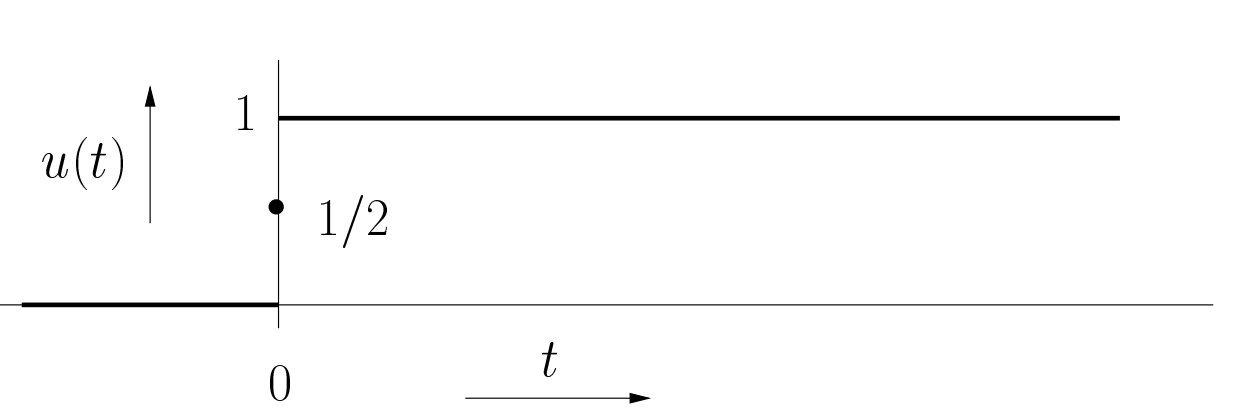
\includegraphics[width = 5cm, valign=t]{include/Wichtige Funktionen/img/Sprungfunktion.png} &
  Sprungfunktion (Heaviside):
  Normierter Einschaltvorgang
  $$H(t) = \begin{cases}
               0 \textrm{ für }  t<0,                                                                      \\
               [\frac{1}{2} \textrm{ für }  t = 0,] \textrm{ \tiny(nicht immer vorhanden; dann 1 für t=0)} \\
               1 \textrm{ für }  t >0.
             \end{cases}   $$
  \\
  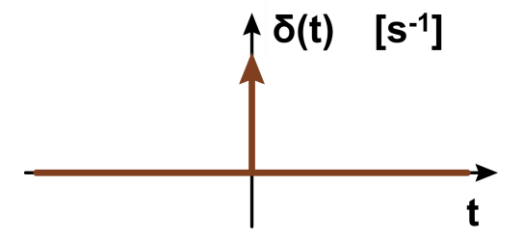
\includegraphics[width = 5cm, valign=t]{include/Wichtige Funktionen/img/Impulsfunktion.png} &
  Diracimpuls \tiny (auch Impuls-/Deltafunktion, Delta-Distribution)
  \normalsize \newline
  Unendlicher kurzer normierter Impuls mit unendlicher Amplitude
  $$\int\limits _{-\infty} ^{+\infty} f(t) \cdot \delta (t-t_0) dt = f(t_0) \;
    \int\limits _{-\infty} ^{+\infty} f(t) \cdot \delta (t) dt = f(0) \;
  \int\limits _{-\infty} ^{+\infty} \delta (t) dt = 1$$                                 \\
  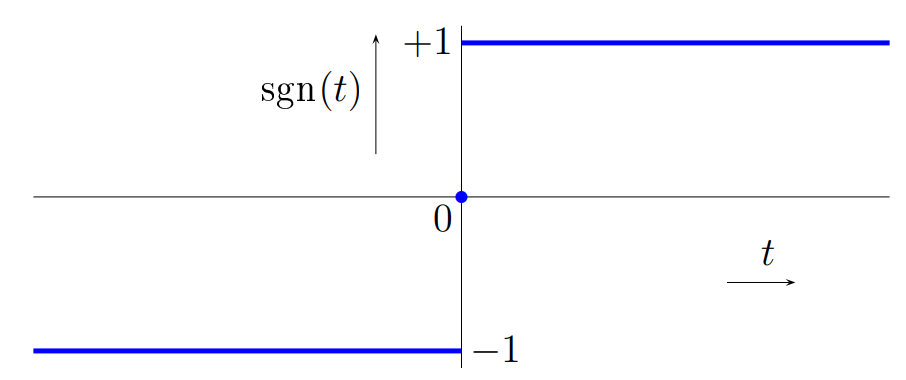
\includegraphics[width = 5cm, valign=t]{include/Wichtige Funktionen/img/Signumfunktion.png} &
  Signumfunktion (Vorzeichenfunktion)
  $$sgn(t) = \begin{cases}
                 -1 \textrm{ für }  t<0,  \\
                 0 \textrm{ für }  t = 0, \\
                 1 \textrm{ für }  t >0.
               \end{cases}   $$                                                   \\
  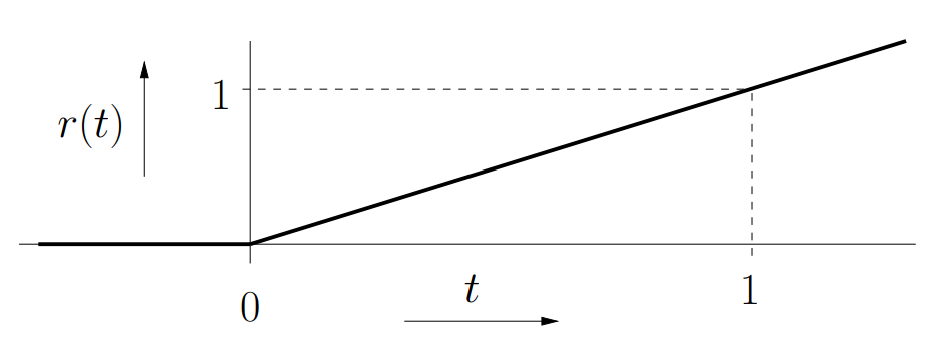
\includegraphics[width=5cm, valign=t]{include/Wichtige Funktionen/img/Rampenfunktion.png}   &
  Rampenfunktion 
  $$r(t) = \begin{cases}
               0 \textrm{ für } t \leq 0, \\
               t \textrm{ für } t > 0.
             \end{cases}$$\\
\end{tabular}

\section{Fourier-Reihe}
\subsubsection*{Formen}
\begin{tabular}{p{4cm}p{15cm}}
  Trigonometrische Form &
  $x(t) = \frac{u_0}{2} + \sum \limits _{n = 1} ^{\infty} u_n \cdot cos(2\pi n f_0 \cdot t) + v_n \cdot sin(2\pi n f_0 \cdot t) $
  \newline $u_n = \frac{2}{T} \int \limits _{T} x(t) \cdot cos(2\pi n f_0 \cdot t)dt$
  $u_n = \frac{2}{T} \int \limits _{T} x(t) \cdot sin(2\pi n f_0 \cdot t)dt$
  \\[20pt]
  Harmonische Form      &
  $x(t) = r_0 + \sum \limits _{n = 1} ^{\infty} r_n \cdot cos(2\pi n f_0 \cdot t + \varpi_n)$
  \newline $r_0 = \frac{u_0}{2} = \frac{1}{T} \int  \limits _{T} x(t) dt $
  $r_n > 0 = \sqrt{u_n^2 + v_n^2}$
  $\varphi = arg(u_n - j \cdot v_n) $
  \\
  Komplexe Form         &
  $x(t) = \sum \limits _{n= -\infty} ^{\infty} c_n \cdot e^{jn2\pi f_0 \cdot t}$
  \newline $c_n = \frac{1}{T} \int \limits _{T} x(t) \cdot e^{-j n 2 \pi f_0 \cdot t} dt$
\end{tabular}

\subsubsection*{Transformation und Rücktransformation}
$$ X(\omega) = \mathcal{F}[x(t)] = \int \limits _{-\infty} ^{+\infty} x(t) \cdot e^{-j \omega t} dt $$
$$ x(t) = \mathcal{F}^{-1}[X(\omega)] = \frac{1}{2 \pi} \int \limits _{- \infty} ^{+ \infty} X(\omega) \cdot e^{j \omega t} d\omega$$



\section{Anhang}

\subsection{Wichtige Werte \& Vereinfachungen}

\subsubsection*{Integration über Periodendauer}
$$\int_T (x \cdot sin(\omega t + \alpha))^2 dt = x^2 \cdot \int_T sin^2(\omega t +\alpha) dt = \frac{x^2}{2}$$
$$\int_T (x \cdot cos(\omega t+\alpha))^2 dt = x^2 \cdot \int_T cos^2(\omega t+\alpha) dt = \frac{x^2}{2}$$


\subsubsection*{Komplex sin/cos}

$$cos \varphi = \frac{e^{j\varphi}+ e^{-j\varphi}}{2}, \; sin \varphi = \frac{e^{j\varphi} - e^{-j\varphi}}{2j} $$

\subsection*{Additionstheoreme}
\begin{multicols}{2}%
$\sin(x\pm y) = \sin(x) \cdot \cos(y) \pm \cos(x) \cdot \sin(y)$
\\$\cos(x \pm y)= \cos(x) \cdot \cos(y) \pm \sin(x) \cdot \sin(y)$
\\$\sin(2x) = 2 \sin(x) \cdot cos(x)$
\\$\cos(2x) = \cos^2(x)-\sin^2(x)$
\\$\sin^2(x) + \cos^2(x) = 1 $
\\$\sin x \; \sin y = \frac{1}{2}(\cos (x-y) - \cos (x+y))$
\\$\cos x \; \cos y = \frac{1}{2}(\cos (x-y) + \cos (x+y)) \sin x\;\cos y={\frac {1}{2}}(\sin(x-y)+\sin(x+y))$
\\$\sin x \; \cos y = \frac{1}{2}(\sin (x-y) + \sin (x+y))$
\\$\sin^2 x = \frac{1}{2}\ (1 - \cos (2x)) $
\\$\cos^2 x = \frac{1}{2}\ (1 + \cos (2x)) $
\end{multicols}


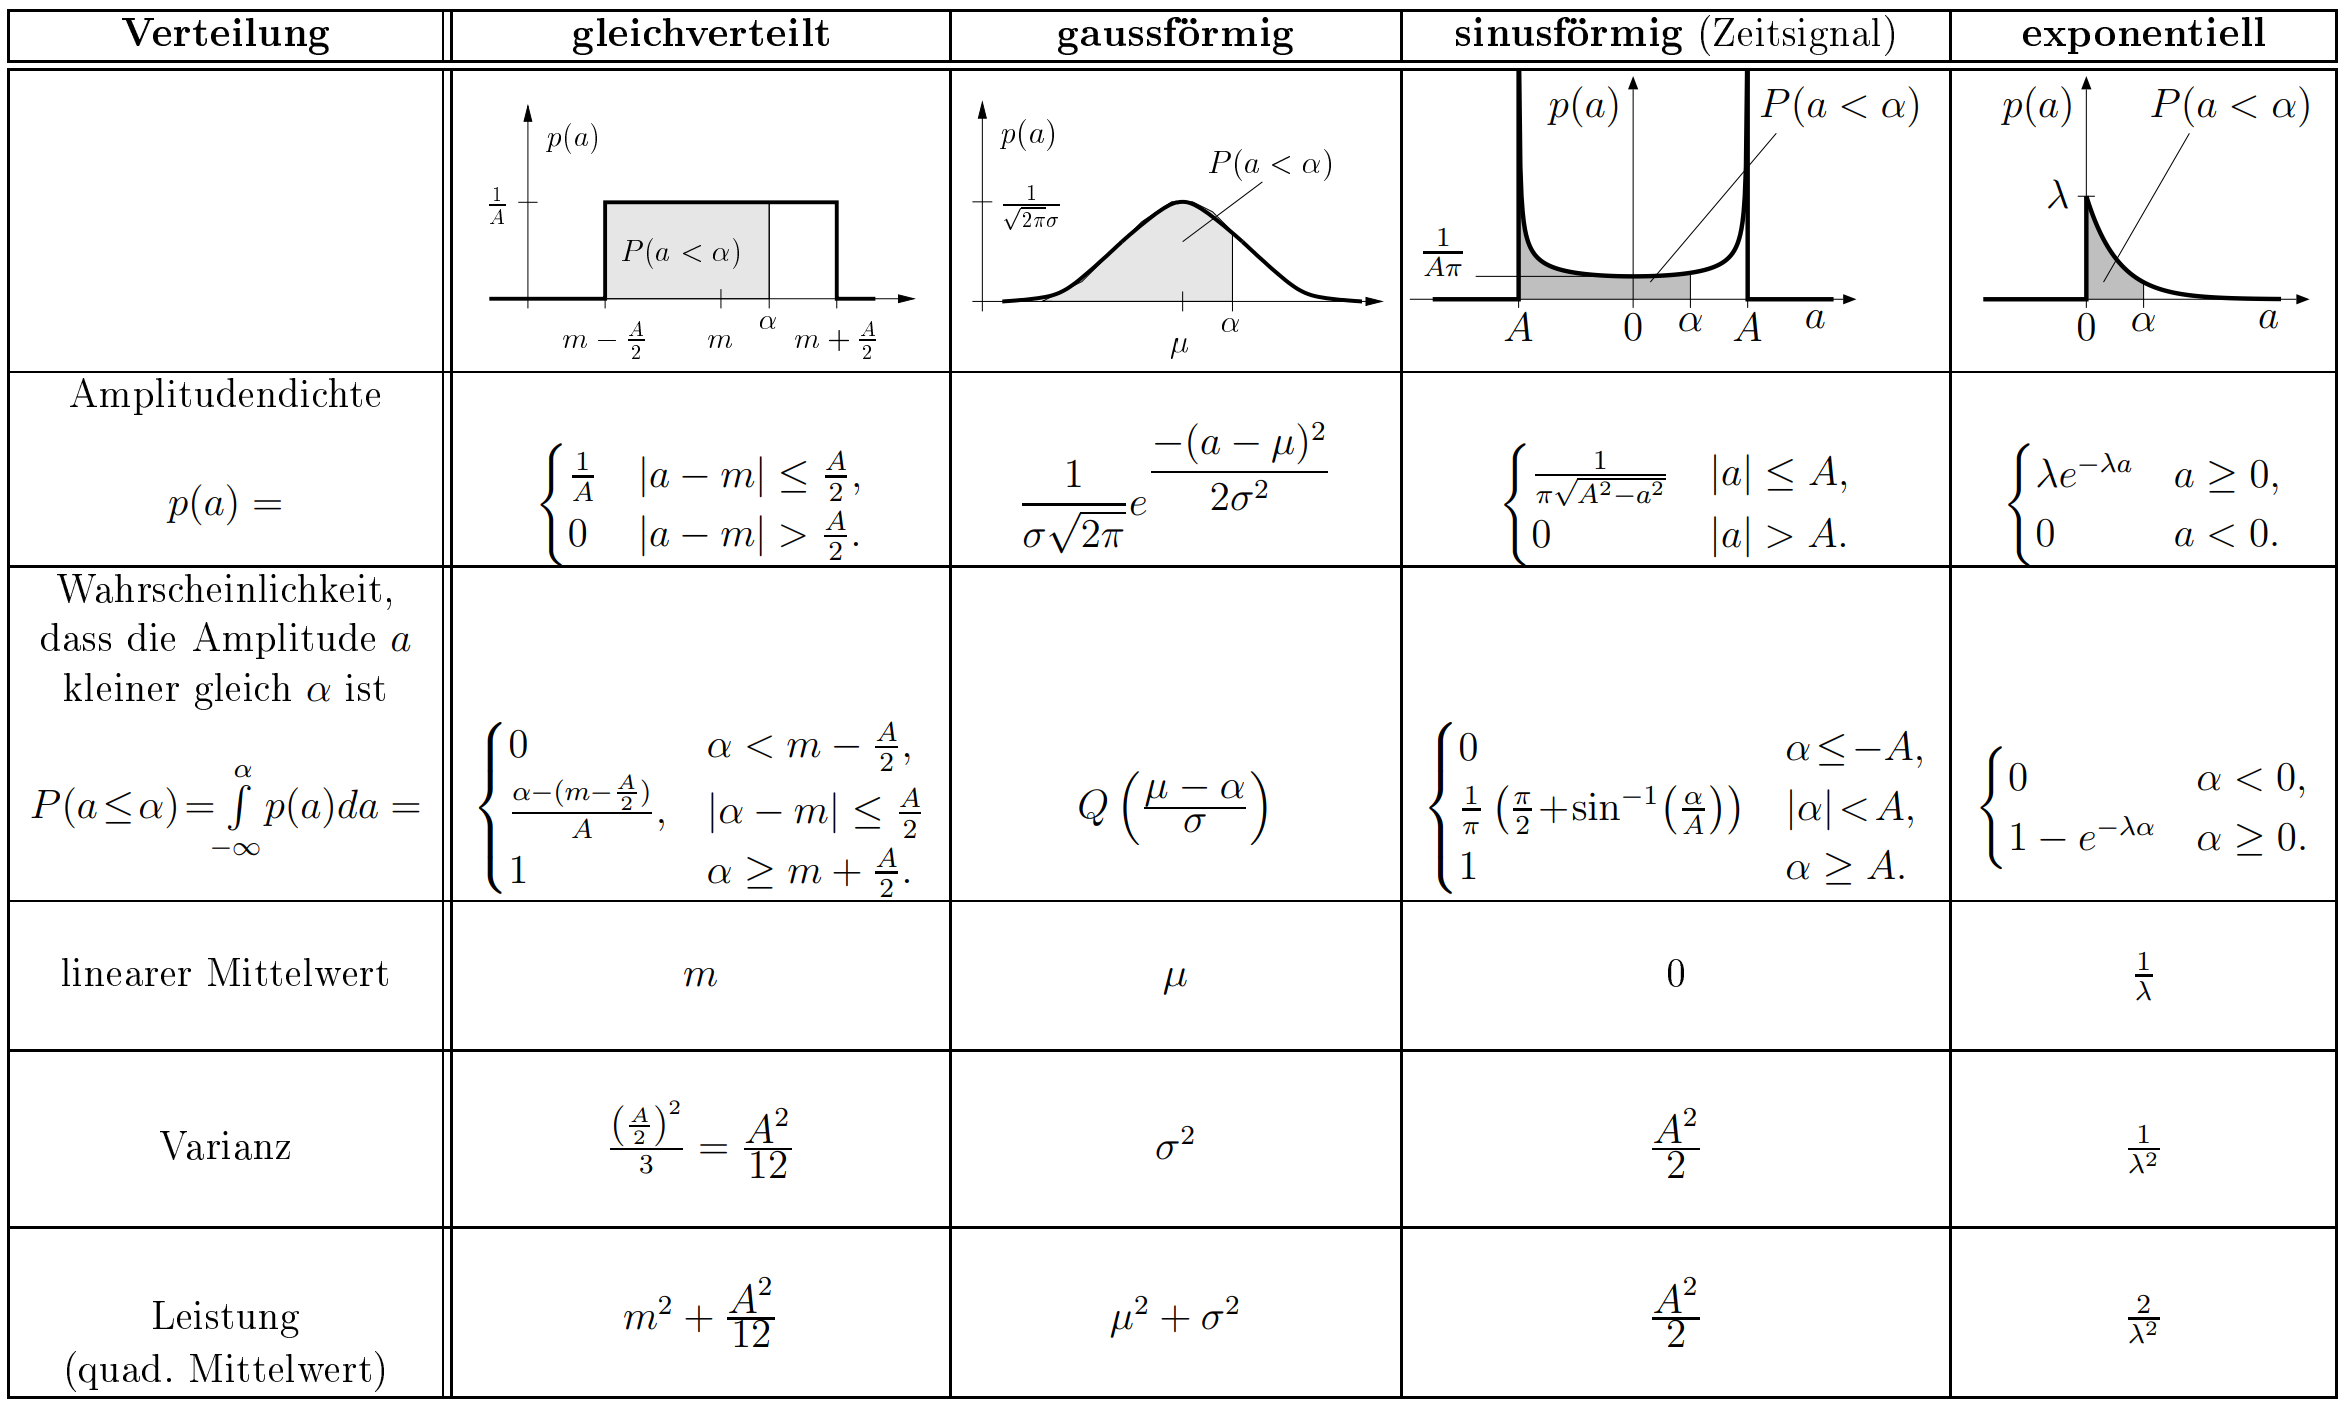
\includegraphics{img/Tabelle_Dichtefunktionen.png}

